\section{Teori}
Denna del av rapporten är ämnad att ge information kring ämnet som behandlas i rapporten. Det som behandlas mer i detalj är 'best practices' men även ledarskap och hur ledarskap kan se ut enligt vissa modeller.
\subsection{Best practice}
Denna rapport har egentligen två huvudbegrepp, 'best practice' och teamledare. 'Best practices' är enligt Oxfords engelska uppslagsverk som "Commercial or professional procedures that are accepted or prescribed as being correct or most effective" \citep{OD}. Löst översatt till svenska betyder detta kommersiella eller professionella tillvägagångssätt vilka är accepterade och föreskrivna som korrekta och mest effektiva. Med andra ord är en 'best practice' det sätt en person på bäst sätt kan utföra en uppgift vilket i fallet som teamledare innebär att genomföra rollen på bästa sätt \citep{itSMF}. En 'best practice' kan till exempel vara att teamledaren väljer att delegera en viss typ av uppgifter till andra gruppmedlemmar eller att teamledaren själv fattar alla beslut gällande en viss fråga. Det finns dock kritiker till 'best practice' konceptet. En av dessa är Eugene Bardach som främst riktar sin kritik mot själva termen 'best practice' på grund av att de kriterier som krävs för att uppfylla en 'best practice' sällan uppfylls. Istället argumenterar han för bra eller smarta practices som till viss del kan bidra till lösningar för vissa situationer \citep{EB}.  
\subsection{Ledarskap}
Det andra begreppet som är av stor betydelse i denna rapport är som tidigare nämnts teamledare. En teamledare kan beskrivas på många sätt men en generell beskrivning är att en teamledare är en gruppmedlem som kan ha viss bestämmanderätt över gruppen men detta är ingen nödvändighet. En teamledare kan antingen vara permanent utsedd eller utsedd under kortare perioder där rollen vandrar mellan olika gruppmedlemmar. Oavsett om teamledaren är permanent utsedd eller inte har denne ett ansvar att representera gruppen utåt samt uppåt vilket betyder att denne kan vara ansvarig gentemot eventuella chefer men teamledaren har även ett ansvar gentemot gruppen i sig. Detta ansvar innebär att teamledaren ska lösa konflikter inom gruppen samt koordinera dess arbete för att uppnå uppsatta mål mål \citep{BD}. 
\newline \newline
När det gäller själva ledarskapet finns det ett antal olika modeller eller stilar. En av dessa togs fram av Kurt Lewin tillsammans med sin forskargrupp under 1930-talet och heter därefter Lewin's Leadership Syles. I studien undersöktes skolbarn som genomförde olika projekt för att se vilka typer av ledarroller som barnen antog. Det man kom fram till var att det fanns tre stilar. En auktoritär, en deltagande eller demokratisk och en delegerande \citep{KAC} vilket illustreras av Figur ~\ref{fig:Lewin}. 
\begin{figure}[H]
\centerline{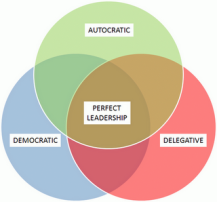
\includegraphics{adam-tex/graphic/leadership}}
\caption{Lewin's Leadership Style}
\label{fig:Lewin}
\end{figure}
\noindent Figuren visar tre cirklar vilka representerar de olika ledarstilarna och att en ledare inte nödvändigtvis behöver tillämpa en av de tre stilarna utan kan tillämpa flera av dem samtidigt. Detta innebär att en riktigt bra ledare, oavsett vilken typ av ledare det rör sig om, har delar av alla tre stilarna för att vid behov kunna använda den som är mest lämpad för situationen. Dock är detta, som tidigare nämnts, en av många modeller för ledarskap men har valts som exempel för att den är generell och lätt att tillämpa på rollen som teamledare.